\documentclass{article}
\usepackage{amsmath}
\usepackage{amssymb}
\usepackage{graphicx}
\usepackage{hyperref}
\usepackage[version=4]{mhchem}


\begin{document}
\section*{Problem}
In triangle \(A B C\), a point \(D\) is taken on \(A B\) and a point \(E\) is taken on \(A C\) such that \(B D: D C=3: 2\), and \(A E: E C=3: 4 . A D\) and \(B E\) intersect at \(M\). Find the area of triangle \(A E M\) if the area of triangle \(A B C\) is 1 .\\
\centering
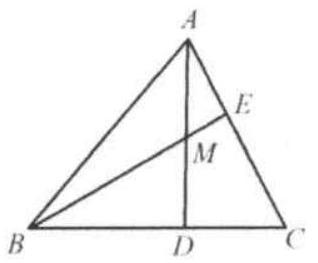
\includegraphics[width=\textwidth]{images/127(3).jpg}

\section*{Solution}
\(\frac{2}{21}\).\\
Draw \(E N / / A D\) to meet \(B C\) at \(N\).\\
Since \(B D: D C=3: 2\) and \(A E: E C=3: 4, N C: D N: B D=8\) : \(6: 21\). So \(E M: M B=6: 21=2: 7\).\\
We know that \(\frac{S_{\triangle A B E}}{S_{\triangle A B C}}=\frac{3}{3+4} \Rightarrow \quad S_{\triangle A B E}=\frac{3}{7} S_{\triangle A B C}=\frac{3}{7}\).\\
\centering
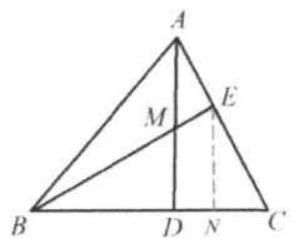
\includegraphics[width=\textwidth]{images/133(2).jpg}


\(S_{\triangle A E M}=\frac{2}{9} S_{\triangle A B E}=\frac{2}{9} \times \frac{3}{7}=\frac{2}{21}\)

\end{document}
